\subsection{Patchplot Library}
\label{sec:lib:patchplots}
\begin{pgfplotslibrary}{patchplots}
	A library for advanced |patch| plots. It has been designed to visualize shaded isoparametric finite element meshes of higher order. Its core is an interface to the generation of smoothly shaped elements with interpolated color values (based on \texttt{.pdf} Shading Type 6 and \texttt{.pdf} Shading Type 7), with additional (limited) support for constant color filling without shadings.

\subsubsection{Additional Patch Types}
\begin{pgfplotskey}{patch type=\mchoice{default,rectangle,triangle,line,bilinear,triangle quadr,biquadratic,coons} (initially default)}
	The |patchplots| library supports several new |patch type|s in addition to the initially available choices (which are |rectangle|,|triangle| and |line|). The documentation of these choices are replicated from page~\pageref{key:patch:type} here.

	The |patchplots| library is especially strong for |shader=interp|, so this is our main focus in the documentation here.

	\paragraph{Attention:} At the time of this writing, many free pdf viewers do not fully support the following shadings\footnote{The author of this package has submitted bugfixes to Linux viewers based on xpdf/libpoppler, so the problem will vanish in the future versions.}. The preferred viewer is Adobe Acrobat Reader.

	The choice \declaretext{rectangle} expects one or more rectangular patches with $n=4$ vertices each. These vertices are either encoded as a matrix or as individual patches (using |mesh input=patches|), in the sequence in which you would connect the vertices:
\begin{codeexample}[]
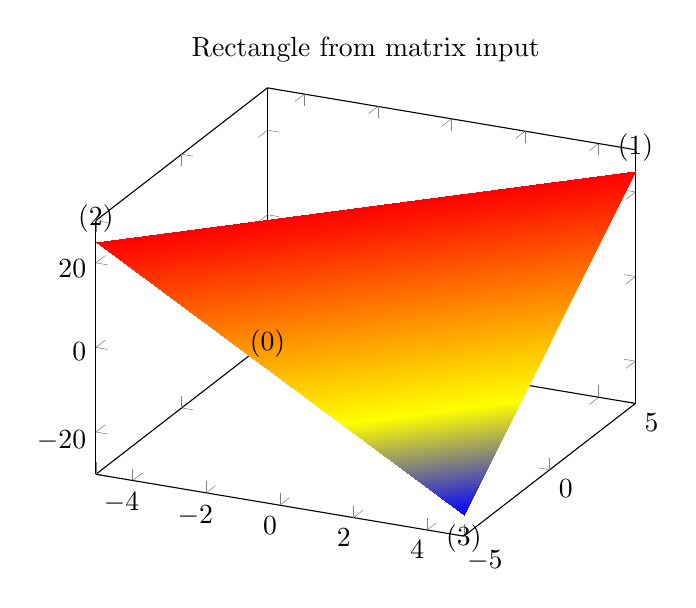
\begin{tikzpicture}
\begin{axis}[nodes near coords={(\coordindex)},
	title=Rectangle from matrix input]
% note that surf implies 'patch type=rectangle'
\addplot3[surf,shader=interp,samples=2,
	patch type=rectangle] 
	{x*y};
\end{axis}
\end{tikzpicture}
\end{codeexample}
\begin{codeexample}[]
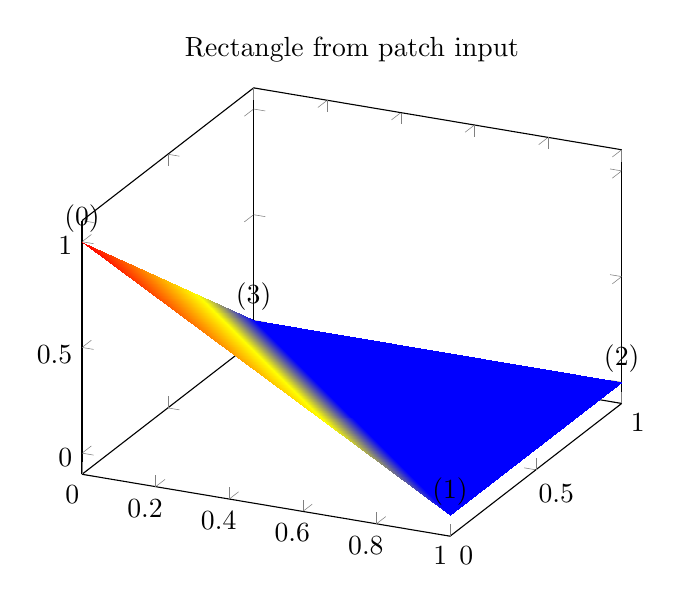
\begin{tikzpicture}
\begin{axis}[nodes near coords={(\coordindex)},
	title=Rectangle from patch input]
\addplot3[patch,shader=interp,patch type=rectangle] coordinates {
	(0,0,1) (1,0,0) (1,1,0) (0,1,0)
};
\end{axis}
\end{tikzpicture}
\end{codeexample}
	\noindent As already documented on page~\pageref{key:patch:type}, the |shader=interp| implementation for |rectangle| uses two triangles and interpolates them linearly.

	The choice \declareandlabel{bilinear} is essentially the same as |rectangular| with respect to its input formats and stroke paths, but it uses correct bilinear shading for |shader=interp|. The two examples from above now become
\begin{codeexample}[]
\begin{tikzpicture}
\begin{axis}[nodes near coords={(\coordindex)},
	title=Bilinear from $2\times 2$ matrix input]
% note that surf implies 'patch type=rectangle'
\addplot3[surf,shader=interp,samples=2,
	patch type=bilinear] 
	{x*y};
\end{axis}
\end{tikzpicture}
\end{codeexample}
\begin{codeexample}[]
\begin{tikzpicture}
\begin{axis}[nodes near coords={(\coordindex)},
	title=Bilinear from $4$--point patch input]
\addplot3[patch,shader=interp,patch type=bilinear] coordinates {
	(0,0,1) (1,0,0) (1,1,0) (0,1,0)
};
\end{axis}
\end{tikzpicture}
\end{codeexample}

	The choice \declaretext{triangle} expects a sequence of linear triangles, each encoded using $n=3$ vertices:
\begin{codeexample}[]
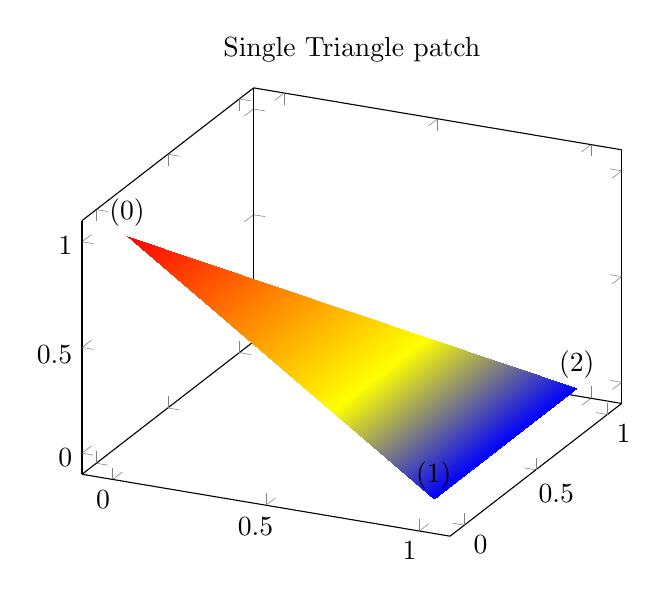
\begin{tikzpicture}
\begin{axis}[enlargelimits,
	nodes near coords={(\coordindex)},
	title=Single Triangle patch]
\addplot3[patch,shader=interp] coordinates {
	(0,0,1)
	(1,0,0)
	(1,1,0)
};
\end{axis}
\end{tikzpicture}
\end{codeexample}

	The choice \declareandlabel{triangle quadr} expects a sequence of isoparametric quadratic triangles, each defined by $n=6$ vertices:
\begin{codeexample}[]
\begin{tikzpicture}
\begin{axis}[nodes near coords={(\coordindex)},
	title=Quadratic Triangle]
\addplot[patch,patch type=triangle quadr,
	shader=interp,point meta=explicit]
coordinates {
	(0,0) [1] (5,4) [2] (0,7) [3]
	(2,3) [1] (3,6) [2] (-1,4)  [3]
};
\end{axis}
\end{tikzpicture}
\end{codeexample}
\begin{codeexample}[]
\begin{tikzpicture}
\begin{axis}[nodes near coords={(\coordindex)},
	title=Quadratic Triangle]
\addplot3[patch,patch type=triangle quadr,
	shader=interp]
coordinates {
	(0,0,1) (5,4,0) (0,7,0)
	(2,3,0) (3,6,0) (-1,4,0)
};
\end{axis}
\end{tikzpicture}
\end{codeexample}
	\noindent Here, the edges have the correct quadratic shape. However, the color interpolation is just \emph{bilinear}; using the color values of the corners and ignoring the rest (consider using |patch refines| to improve the color interpolation). For three dimensions, \PGFPlots\ checks the depth of corners to determine foreground/background. For two dimensions, strongly distorted elements may fold over each other in unexpected ways. 

	The choice \declareandlabel{biquadratic} expects a sequence of isoparametric biquadratic quadrilaterals (rectangles), each defined by $n=9$ vertices:
\begin{codeexample}[]
\begin{tikzpicture}
\begin{axis}[nodes near coords={(\coordindex)},
	title=Single Biquadratic Quadrilateral]
\addplot[patch,patch type=biquadratic,
	shader=interp,point meta=explicit]
coordinates {
	(0,0) [1] (6,1) [2] (5,5) [3] (-1,5) [4]
	(3,1) [1] (6,3) [2] (2,6) [3] (0,3) [4]
	(3,3.75) [4]
};
\end{axis}
\end{tikzpicture}
\end{codeexample}
\begin{codeexample}[]
\begin{tikzpicture}
\begin{axis}[nodes near coords={(\coordindex)},
	title=Single Biquadratic Quadrilateral]
\addplot3[patch,patch type=biquadratic,shader=interp]
coordinates {
	(0,0,1) (6,1,0) (5,5,0) (-1,5,0)
	(3,1,0) (6,3,0) (2,6,0) (0,3,0)
	(3,3.75,0)
};
\end{axis}
\end{tikzpicture}
\end{codeexample}
	\noindent Similar to |triangle quadr|, the edges have the correct quadratic shape -- but the color interpolation is just \emph{bilinear}; using the color values of the corners and ignoring the rest. Again, consider using |patch refines| to improve the color interpolation.

	The choice \declareandlabel{coons} expects a sequence of one or more coons patches, made up of $n=12$ points each. A coons patch is delimited by four cubic Bezier curves, with the end points attached to each other -- and the $n$ points provide the required control points for these curves in a specific ordering which is illustrated in the following example:
\begin{codeexample}[]
\begin{tikzpicture}
\begin{axis}[nodes near coords={(\coordindex)},
	width=12cm,
	title=A Coons Patch]
\addplot[mark=*,patch,patch type=coons,
	shader=interp,point meta=explicit] 
coordinates {
	(0,0)   [0] % first corner
	(1,-1)  [0] % bezier control point between (0) and (3)
	(4,0.7) [0] % bezier control point between (0) and (3)
	%
	(3,2)   [1] % second corner
	(4,3.5) [1] % bezier control point between (3) and (6)
	(7,2)   [1] % bezier control point between (3) and (6)
	%
	(7,1)      [2] % third corner
	(6,0.6)    [2] % bezier control point between (6) and (9)
	(4.5,-0.5) [2] % bezier control point between (6) and (9)
	%
	(5,-2)   [3] % fourth corner
	(4,-2.5) [3] % bezier control point between (9) and (0)
	(-1,-2)  [3] % bezier control point between (9) and (0)
};
\end{axis}
\end{tikzpicture}
\end{codeexample}
	\noindent The four cubic Bezier curves are \emph{equivalent} to \texttt{curveto} paths of \pgfname, i.e.\  \parg{corner 1}|.. controls|\parg{control point A}| and |\parg{control point B}| .. |\parg{corner 2} paths. The interpolated shading is bilinear. More precisely, a bilinear shading in the unit cube $[0,1]^2$ is initialised which is then mapped into the coons patch such that the corners match. The color interpolation uses only the color data of the four corners, color values of intermediate control points are ignored for the shading (although their value will be respected for the upper and lower limit of color data). In contrast to the finite element patches, a coons patch is inherently two--dimensional. While you can still use three--dimensional coordinates, \PGFPlots\ will draw the shading as you provide it, without checkout for the depth information (as it does for the other |patch type|s). In other words: depending on the current |view| angle, the shading might fold over itself in unexpected ways.

	Even for two dimensions, coons patches may fold over themselves. To determine which part is foreground and which part is background, the following rule applies: the four corner points $(0)$, $(3)$, $(6)$, $(9)$ are associated to the unit cube points $(u,v) = (0,0)$, $(0,1)$, $(1,1)$ and $(1,0)$, respectively. The edge between corner $(3)$ and $(6)$ (i.e. the one with $v=1$) is foreground, the edge between $(1)$ and $(9)$ is background. Thus, large values of $v$ are drawn on top of small values of $v$. If $v$ is constant, large values of $u$ are drawn on top of small values of $u$. Thus, reordering the patch vertices (choosing a different first vertex and/or reversing the sequence) allows to get different foreground/background configurations\footnote{Internally, \PGFPlots\ employs such mechanisms to map the higher order isoparametric patch types to coons patches, sorting according their corner's depth information.}.
	
\end{pgfplotskey}



\subsubsection{Automatic Patch Refinement and Triangulation}
\PGFPlots\ supports automatic patch refinement. There are mainly two purposes for patch refinement: to increase the quality of |z buffer=sort| and/or to improve color interpolation for high--order patches. 

\begin{pgfplotskey}{patch refines=\marg{levels} (initially 0)}
	This key controls patch refinement. The initial choice |patch refines=0| disables refinement and visualizes elements as they have been found in input files.

	A positive \meta{levels} enables (recursive) patch refinement: each patch is refined individually. 

	The following example illustrates the |patch refines| feature for a |triangle quadr| shape function on an edge. Note that since \PGFPlots\ uses only first order shading which is based on the corner points $(0)$, $(1)$ and $(2)$, the specified shape function of |patch refines=0| has constant color. Higher \meta{levels} approximate the patch with increasing quality:
\begin{codeexample}[]
\foreach \level in {0,1,2} {%
	\begin{tikzpicture}
	\begin{axis}[
		nodes near coords={(\coordindex)},
		footnotesize,
		title={patch refines=\level}]

	\addplot3[patch,patch type=triangle quadr,
		shader=faceted interp,patch refines=\level]
	coordinates {
		(0,0,0) (5,4,0) (0,7,0)
		(2,3,0) (3,6,1) (-1,4,0)
	};
	\end{axis}
	\end{tikzpicture}
}
\end{codeexample}
	\noindent In this example, patch refinement makes a huge difference since it is just one element with huge displacements. For practical examples, you probably won't need many refinement levels.
	
	The refined patches reproduce the geometry's shape exactly. In addition, they improve color interpolation. Note that its purpose is just visualization, therefor hanging nodes are allowed (and will be generated by |patch refine| for most |patch type|s).

	Patch refinement is implemented for all supported patches except for |patch type=coons|.
\end{pgfplotskey}

\begin{pgfplotskey}{patch to triangles=\mchoice{true,false} (initially false)}
	Occasionally, one has a complicated |patch type| on input and would like to visualize it as a |triangle| mesh. \PGFPlots\ supports automatic triangulation of patches. Triangulation means to replace each individual input patch by one or more triangles. Triangulation can be combined with |patch refines| in which case |patch refines| is applied first and the resulting refined patches are then triangulated.
\begin{codeexample}[]
\foreach \level in {0,1,2} {%
	\begin{tikzpicture}
	\begin{axis}[
		nodes near coords={(\coordindex)},
		footnotesize,
		title={Triangulation + \level\ refines}]

	\addplot3[patch,patch type=biquadratic,shader=faceted interp,
		patch to triangles,patch refines=\level]
	coordinates {
		(0,0,0) (6,1,0) (5,5,0) (-1,5,0)
		(3,1,0) (6,3,0) (2,6,0) (0,3,0)
		(3,3.75,1)
	};
	\end{axis}
	\end{tikzpicture}
}
\end{codeexample}
\end{pgfplotskey}

\subsubsection{Peculiarities of Flat Shading and High Order Patches}
\label{sec:lib:patchplots:flat}
The |patchplots| library has been optimized for use with interpolated shadings, i.e.\ for |shader=interp|: it allows the filled area to fold over itsself or to be outside of the patch boundaries.

\PGFPlots\ also supports |shader=flat| and |shader=faceted| by simply stroking and/or filling the patch boundaries. Naturally, such an approach works only if the enclosed patch boundary and the filled area are essentially the same! Consider using |shader=flat| or |shader=faceted| only if the \emph{mesh width is small enough} such that patches do not fold over themselves.

The following example illustrates the effect: the coarse single element on the left folds over itsself, resulting in strange fill patterns. Refining the mesh reduces the effect.
\begin{codeexample}[]
\foreach \level in {0,1,2} {%
	\begin{tikzpicture}
	\begin{axis}[
		footnotesize,
		title={Faceted + \level\ refines}]

	\addplot3[patch,patch type=biquadratic,shader=faceted,
		patch refines=\level]
	coordinates {
		(0,0,1) (6,1,0) (5,5,0) (-1,5,0)
		(3,1,0) (6,3,0) (2,6,0) (0,3,0)
		(3,3.75,0)
	};
	\end{axis}
	\end{tikzpicture}
}
\end{codeexample}

\subsubsection{Drawing Grids}
The |patchplots| library supports grid (|mesh|) visualizes in the same way as for two/three--dimensional |mesh|- and |surf| plots. This includes four different approaches: the first is |shader=faceted|, which uses constant fill color and |faceted color| for stroke paths (as we already saw in Section~\ref{sec:lib:patchplots:flat}). The second approach is to use |shader=faceted interp| which uses interpolated shadings for filling and issues stroke paths on top of each interpolated element. The third approach is to issue two |\addplot| commands, one with the filled |patch| plot, and one with a |patch,mesh| style which only draws (colored) grid lines on top of the previous plot. The three approaches are shown below.
\begin{codeexample}[]
\begin{tikzpicture}
\begin{axis}[
	title={Grids with shader=faceted}]

\addplot3[patch,patch type=biquadratic,
	shader=faceted,patch refines=3]
coordinates {
	(0,0,1) (6,1,1.6) (5,5,1.3) (-1,5,0)
	(3,1,0) (6,3,0.4) (2,6,1.1) (0,3,0.9)
	(3,3.75,0.5)
};
\end{axis}
\end{tikzpicture}
\end{codeexample}
\noindent As already discussed in Section~\ref{sec:lib:patchplots:flat}, the approach with |shader=faceted| works well if the mesh width is small enough such that single patches do not overlap and their fill area is within the patch boundaries.
%
\begin{codeexample}[]
\begin{tikzpicture}
\begin{axis}[
	title={Grids with shader=faceted interp}]

\addplot3[patch,patch type=biquadratic,
	shader=faceted interp,patch refines=3]
coordinates {
	(0,0,1) (6,1,1.6) (5,5,1.3) (-1,5,0)
	(3,1,0) (6,3,0.4) (2,6,1.1) (0,3,0.9)
	(3,3.75,0.5)
};
\end{axis}
\end{tikzpicture}
\end{codeexample}
\noindent Here, grid lines are defined to be the patch boundary, so it may occasionally happen for coarse patches that grid lines cross the filled area. The |shader=faceted interp| supports |z buffer| -- at the cost of generating one shading for \emph{each} patch element (the stroke path is drawn immediately after the patch element is shaded). This can become quite expensive\footnote{I would really like to hear any well--founded ideas how to improve this issue. In case you have an idea-- let me know!} at display time and may lead to huge pdf files. However, |shader=faceted interp| provides smooth shadings and, at the same time, good  grid lines which are drawn in the correct order. 

%
\begin{codeexample}[]
\begin{tikzpicture}
\begin{axis}[
	title={Mesh on top of patches (i): obscured}]

\addplot3[patch,patch type=biquadratic,shader=interp,
	patch refines=3]
coordinates {
	(0,0,1) (6,1,1.6) (5,5,1.3) (-1,5,0)
	(3,1,0) (6,3,0.4) (2,6,1.1) (0,3,0.9)
	(3,3.75,0.5)
};
\addplot3[patch,patch type=biquadratic,mesh,black,
	patch refines=3]
coordinates {
	(0,0,1) (6,1,1.6) (5,5,1.3) (-1,5,0)
	(3,1,0) (6,3,0.4) (2,6,1.1) (0,3,0.9)
	(3,3.75,0.5)
};
\end{axis}
\end{tikzpicture}
\end{codeexample}
%
\begin{codeexample}[]
\begin{tikzpicture}
\begin{axis}[
	title={Mesh on top of patches (ii): unobscured\\
	  \tiny Geometry provided by Prof. Chernov, Bonn},
	title style={align=center},
	view={156}{28}]
\addplot3[patch,patch type=bilinear,
	shader=interp,
	patch table=plotdata/patchexample_conn.dat] 
	file {plotdata/patchexample_verts.dat};

\addplot3[patch,patch type=bilinear,
	mesh,black,
	patch table=plotdata/patchexample_conn.dat] 
	file {plotdata/patchexample_verts.dat};
\end{axis}
\end{tikzpicture}
\end{codeexample}
\noindent The approach to draw grids separately is realized by means of two |\addplot| statements; the first using |patch| as before, the second using |patch,mesh|. This configures \PGFPlots\ to visualize just the mesh. Make sure you provide `|mesh|' after `|patch|' since the latter actives filled |surf| visualization. The approach of meshes on top of patches implies to draw grid lines simply over any previous drawing operations. Thus, depth information is lost (as displayed in the first example above). Overlaying grid lines on top of the surface works in special cases (see bottom picture). An approach which works always is to provide the mesh at a fixed $z$ position as displayed in the following example:
%
\begin{codeexample}[]
\begin{tikzpicture}
\begin{axis}[
	title={Separate Grids (iii)}]

\addplot3[patch,patch type=biquadratic,shader=interp,
	patch refines=3]
coordinates {
	(0,0,1) (6,1,1.6) (5,5,1.3) (-1,5,0)
	(3,1,0) (6,3,0.4) (2,6,1.1) (0,3,0.9)
	(3,3.75,0.5)
};
\addplot3[patch,patch type=biquadratic,
	mesh,black,
	z filter/.code={\def\pgfmathresult{1.8}},
	patch refines=3]
coordinates {
	(0,0,1) (6,1,1.6) (5,5,1.3) (-1,5,0)
	(3,1,0) (6,3,0.4) (2,6,1.1) (0,3,0.9)
	(3,3.75,0.5)
};
\end{axis}
\end{tikzpicture}
\end{codeexample}
\noindent Here, the first |\addplot3| command is the same as above, just with |shader=interp|. The second reproduces the same geometry, but uses a |z filter| to fix the $z$ coordinate (in this case to $z=1.8$). This effectively overrules all $z$ coordinates.

	Thus, grid lines can be realized either by means of flat fill color with |shader=faceted| (efficient), by means of interpolated fill colors with |shader=faceted interp| (inefficient, see above) or, for special applications, using a separate |patch,mesh| plot which is drawn on top of the patches (efficient). In any case, the mesh visualization considers the |faceted color| which can depend on |mapped color|.

\end{pgfplotslibrary}
